\documentclass[border=5pt]{standalone}
\usepackage{fontspec,xeCJK,amsmath,amssymb,tikz,graphicx}
\usetikzlibrary{arrows.meta,calc}
\setmainfont{Arial}\setCJKmainfont{PingFang SC}
\definecolor{ink}{HTML}{203340}\definecolor{teal}{HTML}{167D88}\definecolor{pale}{HTML}{F0F6F5}\definecolor{warm}{HTML}{A46820}\definecolor{cream}{HTML}{FFF5E4}\definecolor{line}{HTML}{CFDDDF}
% Cropped viewports preserve unmodified built-in imagegen assets.
\newcommand{\scene}[4]{\begin{tikzpicture}\clip(0,0)rectangle(#3,#4);\node[anchor=north west,inner sep=0]at(#1,#2){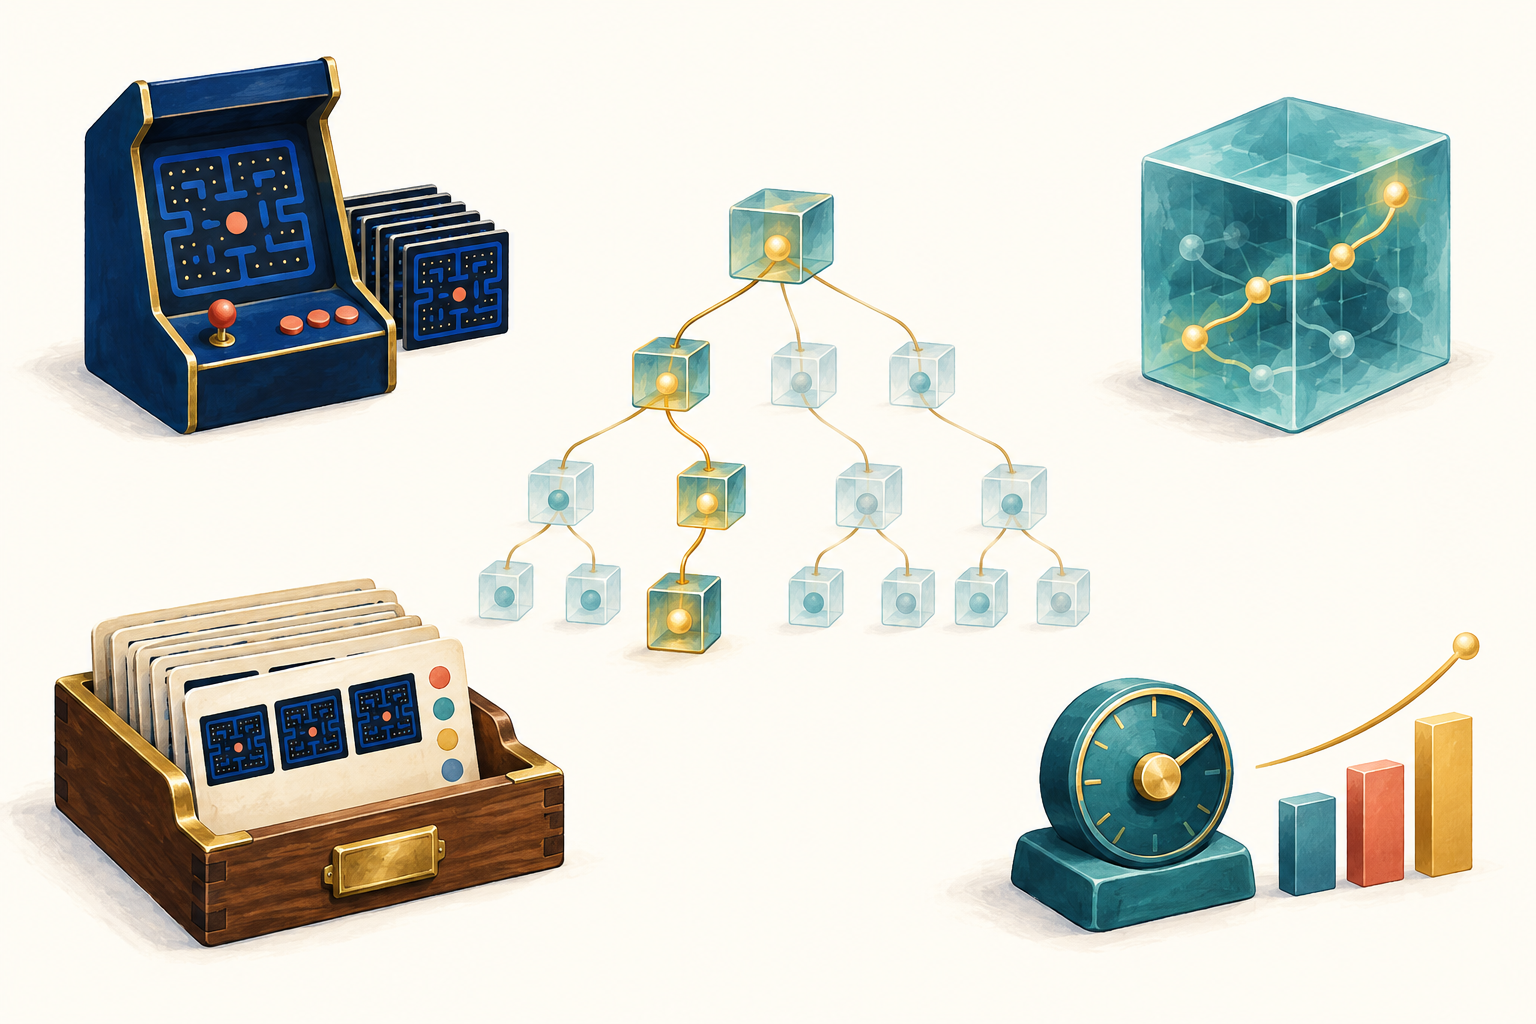
\includegraphics[width=12cm]{muzero-imagegen-draft.png}};\end{tikzpicture}}
\begin{document}
\begin{tikzpicture}[x=1cm,y=1cm,every node/.style={text=ink,font=\fontsize{11}{14}\selectfont},flow/.style={-{Stealth[length=5pt]},draw=teal,line width=1.1pt},learn/.style={-{Stealth[length=5pt]},draw=warm,dashed,line width=1.1pt},box/.style={rounded corners=5pt,draw=line,fill=white}]
\path[use as bounding box](0,0)rectangle(11,30.4);\fill[pale](0,0)rectangle(11,30.4);
\node[font=\fontsize{21}{25}\selectfont\bfseries]at(5.5,29.7){MuZero：学会在脑内试走};
\node[text=teal]at(5.5,29.0){蓝线：决策与交互　　金色虚线：训练与更新};
\draw[box](.35,24.0)rectangle(10.65,28.5);
\node[anchor=west,font=\fontsize{14}{17}\selectfont\bfseries]at(.65,28.0){A　真实输入 → 压成任务相关状态};
\node at(2.4,26.3){\resizebox{3.2cm}{!}{\scene{0}{3.55}{4.1}{3.2}}};
\node[align=left,anchor=west]at(4.65,26.6){观测历史 $o_{1:t}$\quad$\xrightarrow{\ h_\theta\ }\ s_t^0$\\[8pt]Atari：$96\times96\times128$\\[6pt]$\to 6\times6\times256$};
\node[font=\fontsize{10}{13}\selectfont]at(5.5,24.55){32 帧 RGB + 32 个动作平面；真实走一步，就重新编码观测};
\draw[flow](5.5,24.0)--(5.5,23.55);
\draw[box](.35,18.0)rectangle(10.65,23.55);
\node[anchor=west,font=\fontsize{14}{17}\selectfont\bfseries]at(.65,23.0){B　同一组 $g,f$，反复推演假想动作};
\node at(2.1,21.0){\resizebox{2.5cm}{!}{\scene{-8.55}{3.5}{3.1}{2.85}}};
\node[align=left,anchor=west]at(4.15,21.25){$(r_t^k,s_t^k)=g_\theta(s_t^{k-1},a_{t+k})$\\[10pt]$(p_t^k,v_t^k)=f_\theta(s_t^k)$};
\node[align=center]at(5.5,19.45){$r$：这步奖励　$p$：动作先验　$v$：后续回报\\[5pt]隐藏状态 $s$ 留给下一次推演；不生成未来像素};
\node[font=\fontsize{10}{13}\selectfont,text=teal]at(5.5,18.55){树内分支共享模型参数；搜索本身不更新 $\theta$};
\draw[flow](5.5,18.0)--(5.5,17.55);
\draw[box](.35,11.15)rectangle(10.65,17.55);
\node[anchor=west,font=\fontsize{14}{17}\selectfont\bfseries]at(.65,17.0){C　树搜索 → 选动作 → 真实走一步};
\node at(2.8,14.65){\resizebox{3.9cm}{!}{\begin{tikzpicture}\clip(0,0) --(4.95,0)--(4.95,4.0)--(.7,4.0)--(.7,1.7)--(0,1.7)--cycle;\node[anchor=north west,inner sep=0]at(-3.6,5.25){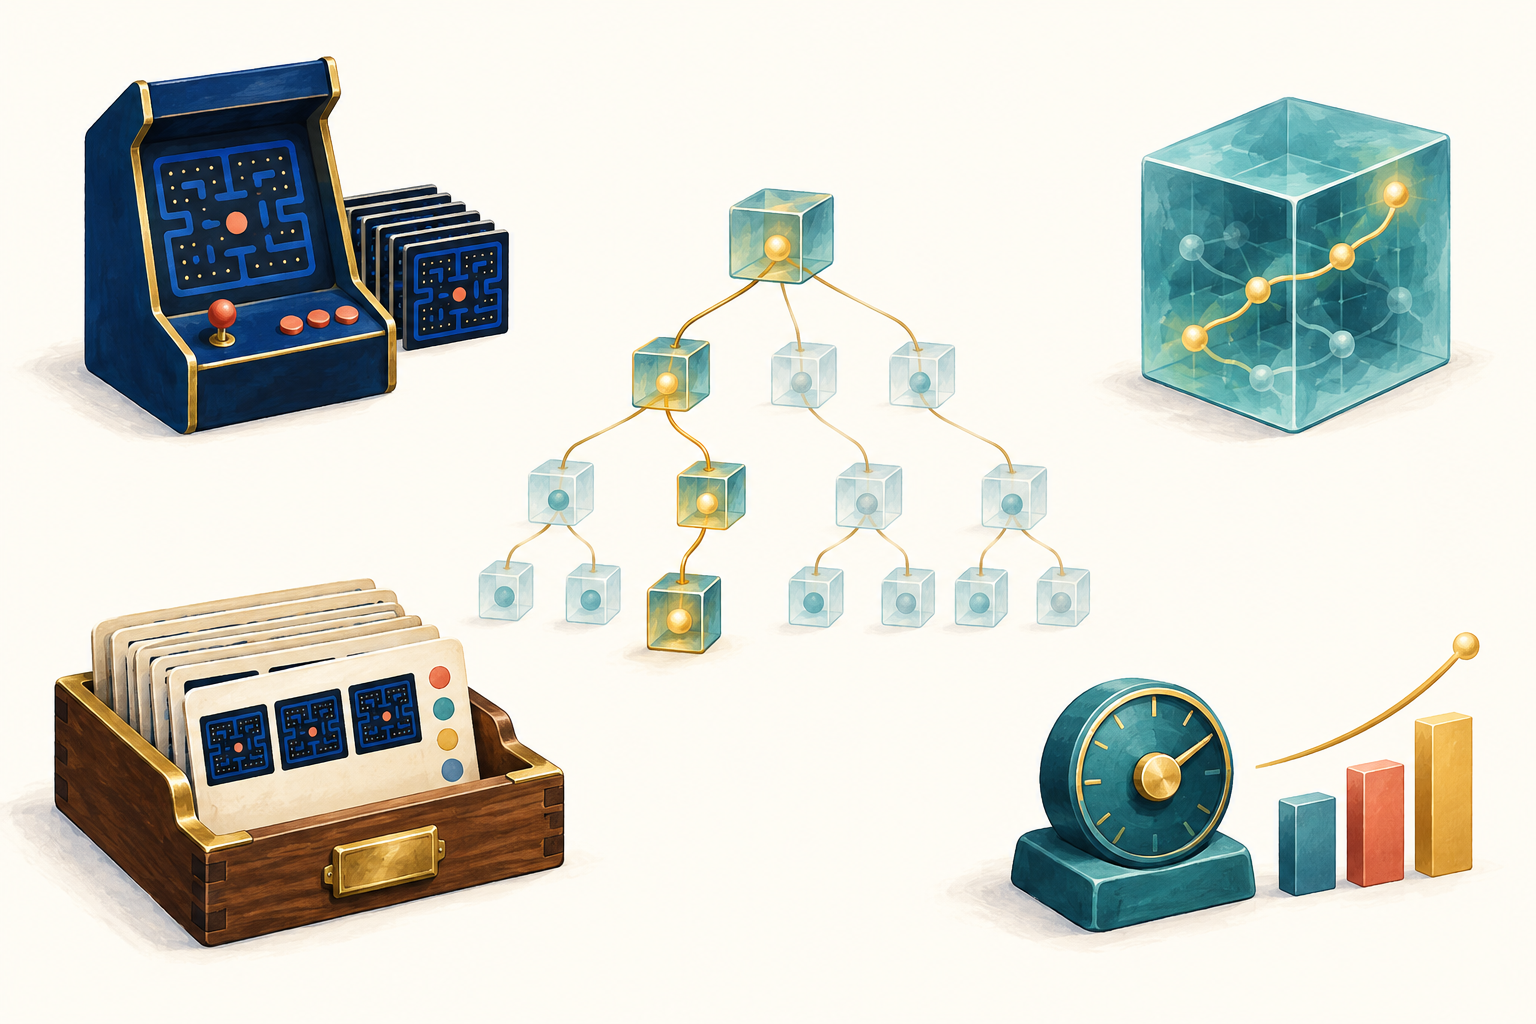
\includegraphics[width=12cm]{muzero-imagegen-draft.png}};\end{tikzpicture}}};
\node[align=left,anchor=west]at(5.35,15.15){选择：$Q$ 与先验 $P$ 平衡\\[8pt]展开：调用 B 得 $r,s,p,v$\\[8pt]回传：$G\leftarrow r+\gamma G$\\[8pt]计数：更新边上的 $N,Q$};
\node at(5.5,12.3){访问次数 $N$ → 搜索策略 $\pi_t$ → 执行 $a_{t+1}$};
\node[font=\fontsize{10}{13}\selectfont]at(5.5,11.65){环境返回 $o_{t+1},u_{t+1}$；带着真实反馈回到 A};
\draw[flow](10.35,12.3)--(10.92,12.3)--(10.92,25.05)--(10.65,25.05);
\draw[learn](5.5,11.15)--(5.5,10.7);
\draw[box,fill=cream](.35,3.5)rectangle(10.65,10.7);
\node[anchor=west,font=\fontsize{14}{17}\selectfont\bfseries]at(.65,10.15){D　回放训练｜把搜索经验教回网络};
\node at(2.4,8.3){\resizebox{3.7cm}{!}{\begin{tikzpicture}\clip(0,0)--(4.3,0)--(4.3,2.35)--(3.4,2.35)--(3.4,3.0)--(0,3.0)--cycle;\node[anchor=north west,inner sep=0]at(-.15,7.5){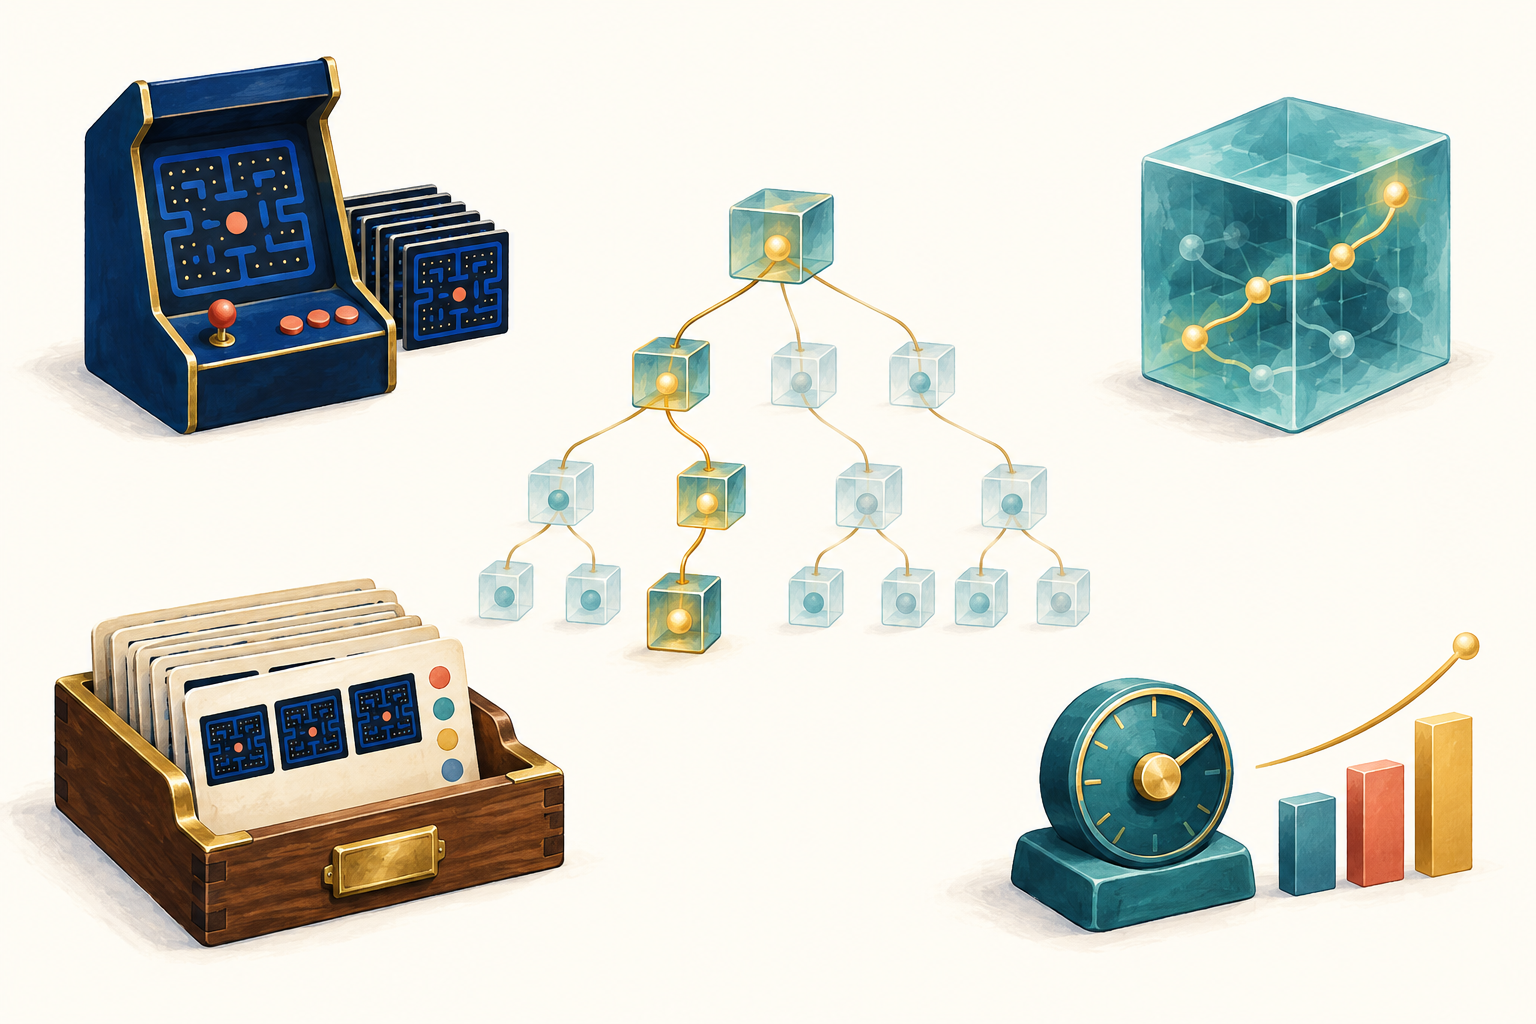
\includegraphics[width=12cm]{muzero-imagegen-draft.png}};\end{tikzpicture}}};
\node[align=left,anchor=west]at(5.05,8.6){存观测、真实动作/奖励\\[8pt]以及搜索 $\pi,\nu$\\[8pt]抽片段，沿真实动作\\[5pt]展开 $K=5$ 步};
\node at(5.5,6.2){$r_t^k\to u_{t+k}$\quad $p_t^k\to\pi_{t+k}$\quad $v_t^k\to z_{t+k}$};
\node at(5.5,5.35){$z_t=\sum_{i=1}^{n}\gamma^{i-1}u_{t+i}+\gamma^n\nu_{t+n}$};
\node[font=\fontsize{10}{13}\selectfont]at(5.5,4.6){奖励 / 策略 / 价值误差，沿展开链反传，共同更新 $h,g,f$};
\node[font=\fontsize{10}{13}\selectfont,text=warm]at(5.5,3.95){Atari：$n=10,\gamma=0.997$；训练 5 步不等于只能搜索 5 层};
\draw[learn](.65,5.5)--(.07,5.5)--(.07,22.0)--(.35,22.0);
\draw[learn](.07,22.0)--(.07,26.3)--(.35,26.3);
\node[font=\fontsize{13}{16}\selectfont\bfseries]at(5.5,2.65){E　验证：玩得好、搜得值、数据花得少？};
\node[font=\fontsize{10}{13}\selectfont]at(5.5,1.85){Fig. 2 / Table 1：分数与预算　Fig. 3 / S3：搜索和训练消融};
\node[font=\fontsize{10}{13}\selectfont]at(5.5,1.12){文章 §1–2：为什么　§3.1–3.4：A/B/C　§3.5–3.7：D};
\node[font=\fontsize{10}{13}\selectfont]at(5.5,.5){§4：E　§5：把任务相关模型的思路带回机器人};
\end{tikzpicture}\end{document}
